\documentclass[aspectratio=169]{beamer}
\usetheme{default}
\usecolortheme{default}
\usepackage{graphicx}
\usepackage{adjustbox}
\usepackage{xcolor}
\usepackage{pgfplots}
\pgfplotsset{compat=1.18}

\setbeamertemplate{navigation symbols}{}

\begin{document}

% Slide 1
\begin{frame}
\centering
\vfill
{\Huge Strange Evals}
\vfill
\end{frame}

% Slide 2
\begin{frame}{Why?}
\begin{itemize}
\item Benchmark scores give a ten-thousand foot view of capability; this group is all about building more powerful and nuanced intuitions of capability
\end{itemize}
\end{frame}

% Slide 3
\begin{frame}{Example}
\centering
\vfill
The stated goal of MMMU, the most cited vision benchmark, is to understand how close a model is to performing at the same level as ``skilled adults''.

\vspace{1em}
{\scriptsize Yue et al., ``MMMU: A Massive Multi-discipline Multimodal Understanding and Reasoning Benchmark for Expert AGI,'' CVPR 2024. Section 1 (Introduction).}
\vfill
\end{frame}

% Slide 4 - Random examples (questions)
\begin{frame}{MMMU Pro -- 5 Random Examples}
\begin{columns}[T]
\column{0.19\textwidth}
\centering
\adjustbox{max width=\textwidth, max height=1.5cm}{\includegraphics{../brokenevals-vlm/mmmu_pro/examples/115_image_0.png}}\\[0.2em]
{\fontsize{4.5}{5.4}\selectfont\raggedright The diagram above depicts iron filings sprinkled around three permanent magnets. Pole R is the same pole as\par}
\vspace{0.1em}
{\fontsize{3}{3.6}\selectfont\raggedright A) Y and Z\\B) X and T\\C) R and T\\D) X and Y\\E) T and Z\\F) T and Y\\G) R and Z\\H) R and Y\\I) X and Z\par}

\column{0.19\textwidth}
\centering
\adjustbox{max width=\textwidth, max height=1.5cm}{\includegraphics{../brokenevals-vlm/mmmu_pro/examples/263_image_0.png}}\\[0.2em]
{\fontsize{4.5}{5.4}\selectfont\raggedright What is your opinion on the fact that certain large insects act as predators of pests? Are they allies or enemies in your view?\par}
\vspace{0.1em}
{\fontsize{3}{3.6}\selectfont\raggedright A) Neutral; it doesn't affect the crops positively or negatively.\\B) Symbiotic; it has a mutual relationship with the crops.\\C) Vector; it is not a pest directly but spreads viruses which damage yield.\\D) Threat; it may not harm the crops directly, but its presence could attract other pests.\\E) Beneficial; it helps in biological control of pests.\\F) Neither; this large insect is not a problem, nor is it a beneficial.\\G) I don't know and don't want to guess.\\H) Friend; this is clearly a predator of pests.\\I) Foe; this is a pest of crops.\\J) Parasitic; it feeds on the pests but also harms the crops.\par}

\column{0.19\textwidth}
\centering
\adjustbox{max width=\textwidth, max height=1.5cm}{\includegraphics{../brokenevals-vlm/mmmu_pro/examples/152_image_0.png}}\\[0.2em]
{\fontsize{4.5}{5.4}\selectfont\raggedright Refer to the figure, which term best describes the practice where members create the visual essence of a chapter on a three-foot strip of paper, discuss it, and then assemble the strips into the shape of sun rays?\par}
\vspace{0.1em}
{\fontsize{3}{3.6}\selectfont\raggedright A) Chapter Ray\\B) Story Ray\\C) Narrative Ray\\D) Magical Realism Ray\\E) Plot Ray\\F) Animal Fantasy Ray\\G) Folklore Ray\\H) Trickster Tale Ray\\I) Fiction Ray\\J) Fable Ray\par}

\column{0.19\textwidth}
\centering
\adjustbox{max width=\textwidth, max height=1.5cm}{\includegraphics{../brokenevals-vlm/mmmu_pro/examples/354_image_0.png}}\\[0.2em]
{\fontsize{4.5}{5.4}\selectfont\raggedright The overall Chi-square value was\par}
\vspace{0.1em}
{\fontsize{3}{3.6}\selectfont\raggedright A) 1196.29\\B) 1700.21\\C) 1300.54\\D) 1567.34\\E) 1082.76\\F) 1552.34\\G) 1203.82\\H) 1100.65\\I) 987.45\\J) 1356.98\par}

\column{0.19\textwidth}
\centering
\adjustbox{max width=\textwidth, max height=1.5cm}{\includegraphics{../brokenevals-vlm/mmmu_pro/examples/402_image_0.png}}\\[0.2em]
{\fontsize{4.5}{5.4}\selectfont\raggedright An all-equity firm is considering the following projects: The T-bill rate is 3.5 percent, and the expected return on the market is 11 percent. Which projects would be incorrectly accepted or rejected if the firm's overall cost of capital was used as a hurdle rate?\par}
\vspace{0.1em}
{\fontsize{3}{3.6}\selectfont\raggedright A) Project Z would be incorrectly rejected; Project Y would be incorrectly accepted.\\B) Project Z would be incorrectly accepted; Project X would be incorrectly rejected.\\C) Project X would be incorrectly rejected; Project Y would be incorrectly accepted.\\D) Project X would be incorrectly accepted; Project Y would be incorrectly rejected.\\E) No project would be incorrectly rejected; Project X would be incorrectly accepted.\\F) Project Y would be incorrectly rejected; Project X would be incorrectly accepted.\\G) No project would be incorrectly rejected; Project Z would be incorrectly accepted.\\H) Project X would be incorrectly rejected; Project Z would be incorrectly accepted.\\I) Project Y would be incorrectly rejected; Project Z would be incorrectly accepted.\\J) Project Z would be incorrectly rejected; Project X would be incorrectly accepted.\par}
\end{columns}
\end{frame}

% Slide 5 - Same images with answers revealed
\begin{frame}{MMMU Pro -- Answers}
\begin{columns}[T]
\column{0.19\textwidth}
\centering
\adjustbox{max width=\textwidth, max height=1.5cm}{\includegraphics{../brokenevals-vlm/mmmu_pro/examples/115_image_0.png}}\\[0.2em]
{\fontsize{4.5}{5.4}\selectfont\raggedright The diagram above depicts iron filings sprinkled around three permanent magnets. Pole R is the same pole as\par}
\vspace{0.1em}
{\fontsize{3}{3.6}\selectfont\raggedright A) Y and Z\\B) X and T\\C) R and T\\\colorbox{green!40}{\textbf{D) X and Y}}\\E) T and Z\\F) T and Y\\G) R and Z\\H) R and Y\\I) X and Z\par}

\column{0.19\textwidth}
\centering
\adjustbox{max width=\textwidth, max height=1.5cm}{\includegraphics{../brokenevals-vlm/mmmu_pro/examples/263_image_0.png}}\\[0.2em]
{\fontsize{4.5}{5.4}\selectfont\raggedright What is your opinion on the fact that certain large insects act as predators of pests? Are they allies or enemies in your view?\par}
\vspace{0.1em}
{\fontsize{3}{3.6}\selectfont\raggedright A) Neutral; it doesn't affect the crops positively or negatively.\\B) Symbiotic; it has a mutual relationship with the crops.\\C) Vector; it is not a pest directly but spreads viruses which damage yield.\\D) Threat; it may not harm the crops directly, but its presence could attract other pests.\\E) Beneficial; it helps in biological control of pests.\\F) Neither; this large insect is not a problem, nor is it a beneficial.\\G) I don't know and don't want to guess.\\H) Friend; this is clearly a predator of pests.\\\colorbox{green!40}{\textbf{I) Foe; this is a pest of crops.}}\\J) Parasitic; it feeds on the pests but also harms the crops.\par}

\column{0.19\textwidth}
\centering
\adjustbox{max width=\textwidth, max height=1.5cm}{\includegraphics{../brokenevals-vlm/mmmu_pro/examples/152_image_0.png}}\\[0.2em]
{\fontsize{4.5}{5.4}\selectfont\raggedright Refer to the figure, which term best describes the practice where members create the visual essence of a chapter on a three-foot strip of paper, discuss it, and then assemble the strips into the shape of sun rays?\par}
\vspace{0.1em}
{\fontsize{3}{3.6}\selectfont\raggedright A) Chapter Ray\\\colorbox{green!40}{\textbf{B) Story Ray}}\\C) Narrative Ray\\D) Magical Realism Ray\\E) Plot Ray\\F) Animal Fantasy Ray\\G) Folklore Ray\\H) Trickster Tale Ray\\I) Fiction Ray\\J) Fable Ray\par}

\column{0.19\textwidth}
\centering
\adjustbox{max width=\textwidth, max height=1.5cm}{\includegraphics{../brokenevals-vlm/mmmu_pro/examples/354_image_0.png}}\\[0.2em]
{\fontsize{4.5}{5.4}\selectfont\raggedright The overall Chi-square value was\par}
\vspace{0.1em}
{\fontsize{3}{3.6}\selectfont\raggedright A) 1196.29\\B) 1700.21\\C) 1300.54\\D) 1567.34\\\colorbox{green!40}{\textbf{E) 1082.76}}\\F) 1552.34\\G) 1203.82\\H) 1100.65\\I) 987.45\\J) 1356.98\par}

\column{0.19\textwidth}
\centering
\adjustbox{max width=\textwidth, max height=1.5cm}{\includegraphics{../brokenevals-vlm/mmmu_pro/examples/402_image_0.png}}\\[0.2em]
{\fontsize{4.5}{5.4}\selectfont\raggedright An all-equity firm is considering the following projects: The T-bill rate is 3.5 percent, and the expected return on the market is 11 percent. Which projects would be incorrectly accepted or rejected if the firm's overall cost of capital was used as a hurdle rate?\par}
\vspace{0.1em}
{\fontsize{3}{3.6}\selectfont\raggedright A) Project Z would be incorrectly rejected; Project Y would be incorrectly accepted.\\B) Project Z would be incorrectly accepted; Project X would be incorrectly rejected.\\C) Project X would be incorrectly rejected; Project Y would be incorrectly accepted.\\D) Project X would be incorrectly accepted; Project Y would be incorrectly rejected.\\E) No project would be incorrectly rejected; Project X would be incorrectly accepted.\\F) Project Y would be incorrectly rejected; Project X would be incorrectly accepted.\\G) No project would be incorrectly rejected; Project Z would be incorrectly accepted.\\\colorbox{green!40}{\textbf{H) Project X would be incorrectly rejected; Project Z would be incorrectly accepted.}}\\I) Project Y would be incorrectly rejected; Project Z would be incorrectly accepted.\\J) Project Z would be incorrectly rejected; Project X would be incorrectly accepted.\par}
\end{columns}
\end{frame}

% Slide 6 - ZeroBench example
\begin{frame}{Cherry Picked ZeroBench Example}
\centering
\adjustbox{max width=0.6\textwidth, max height=0.55\textheight}{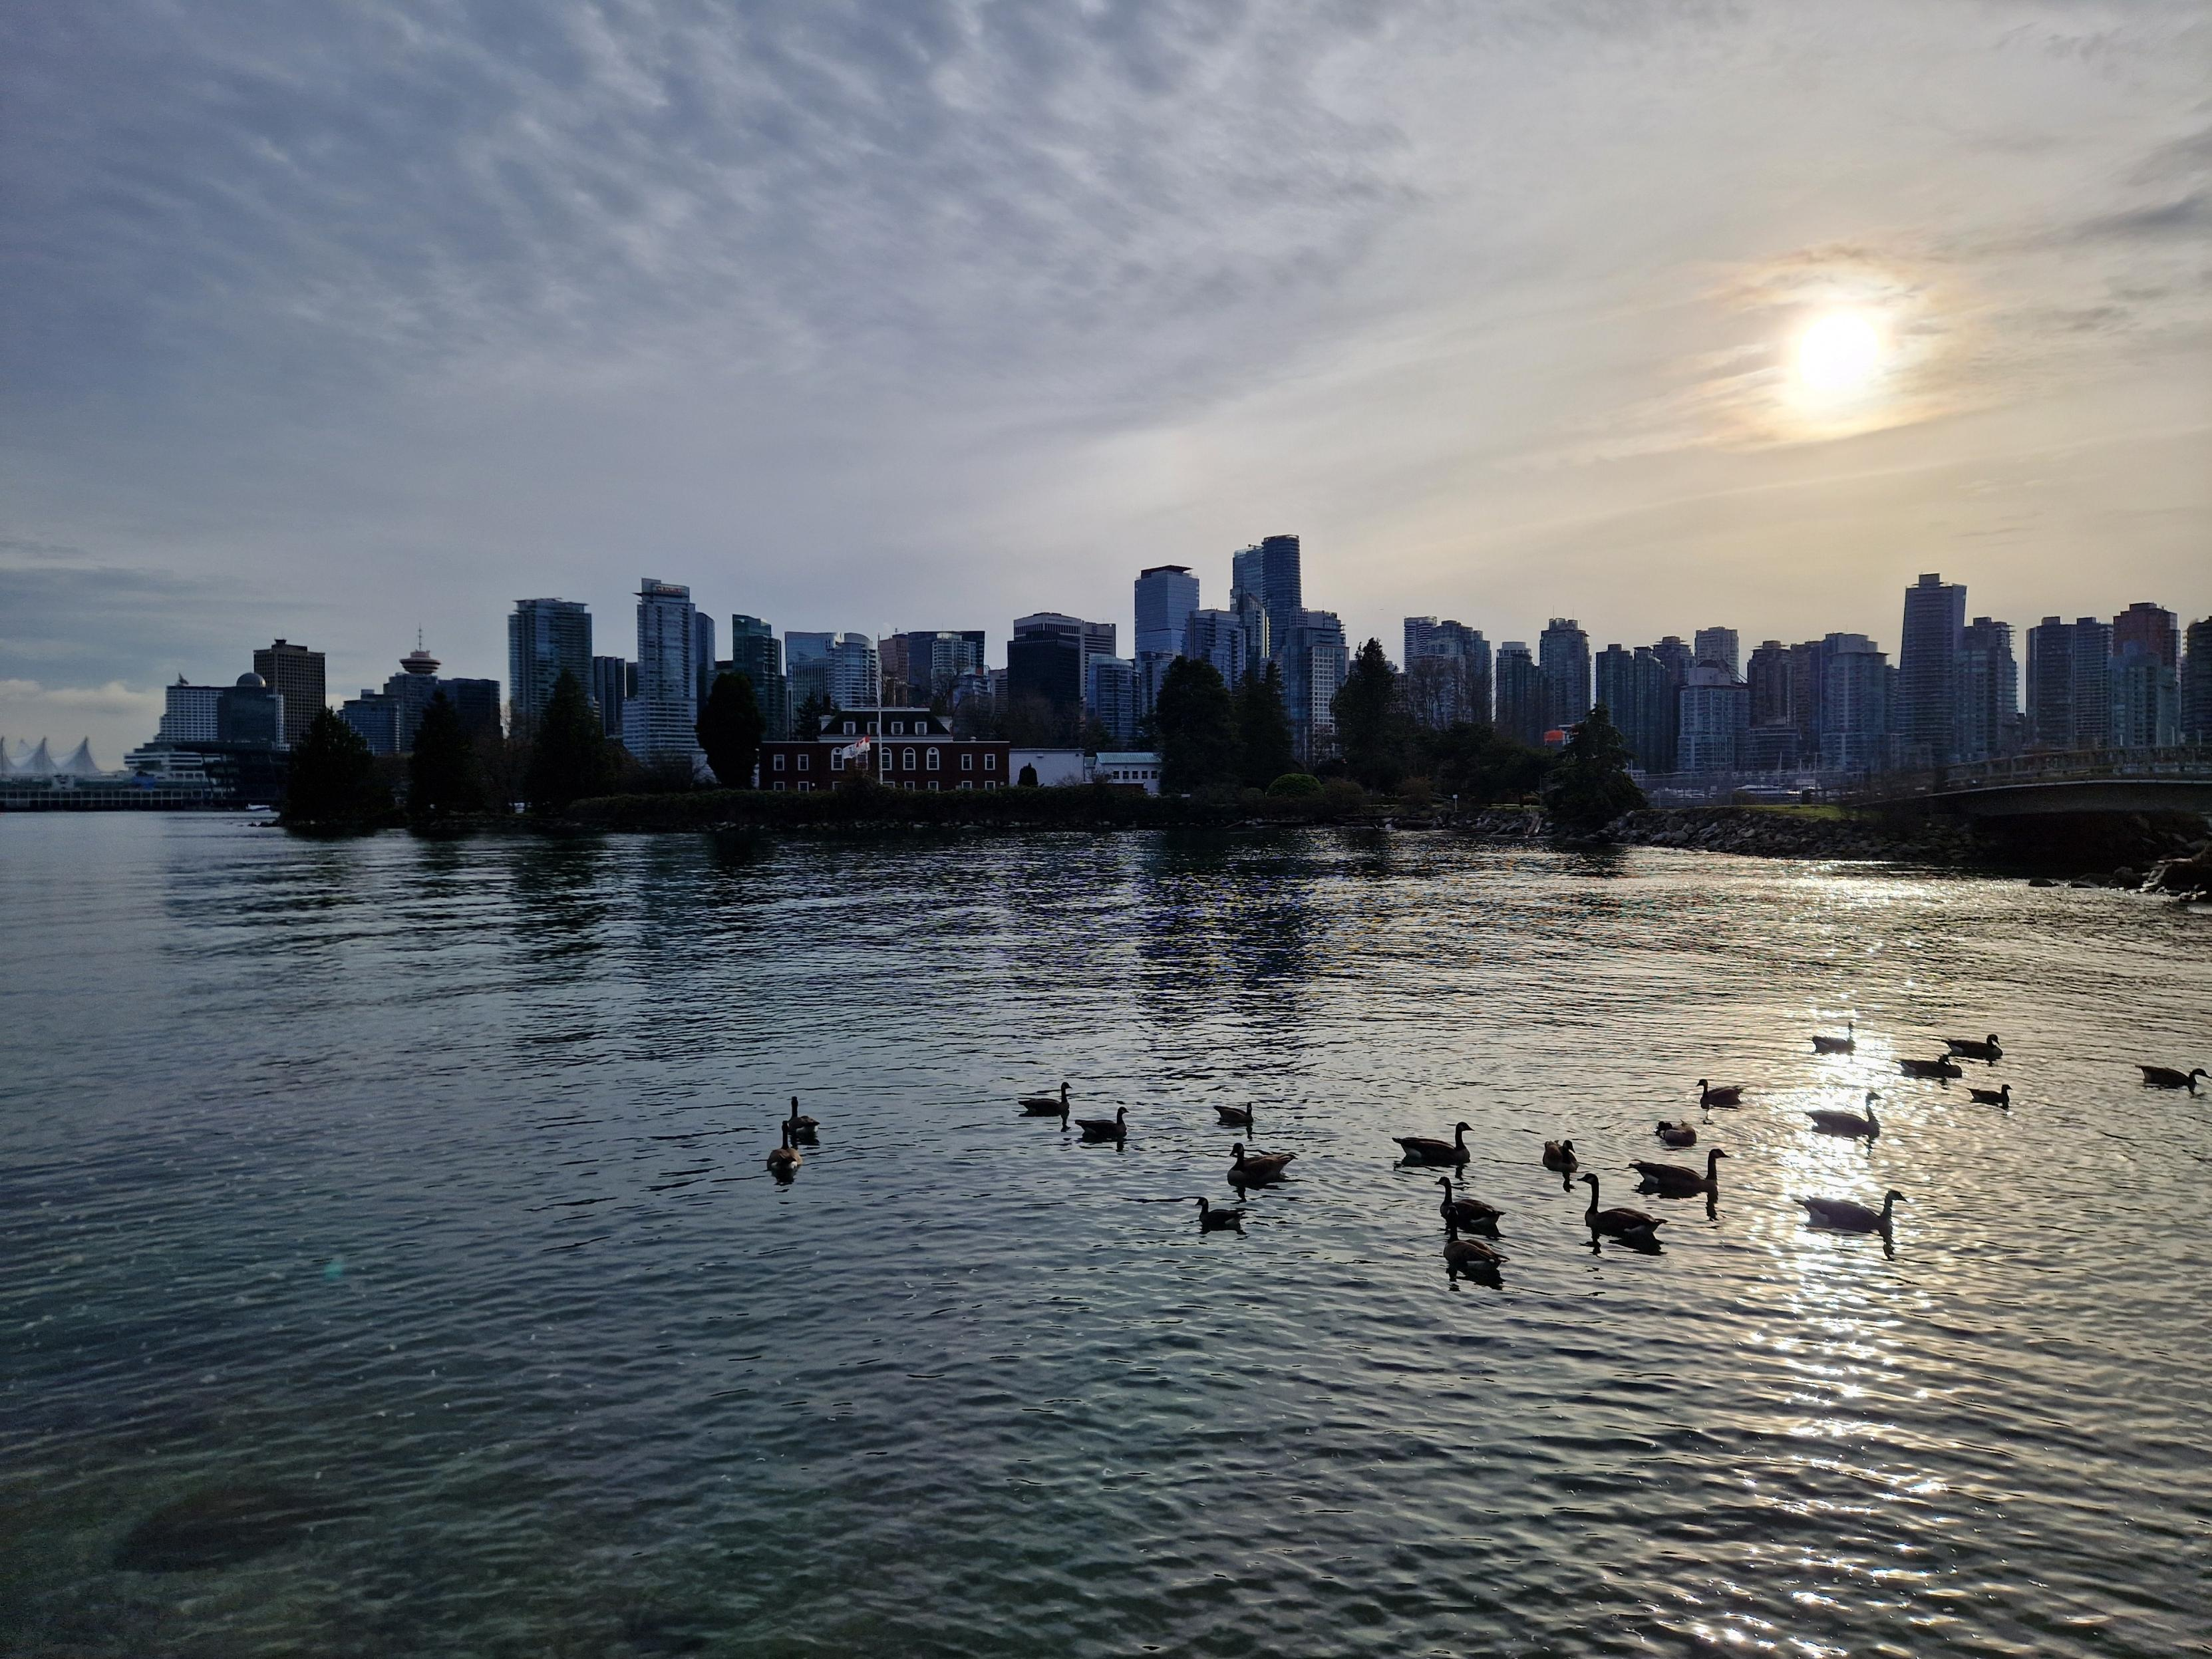
\includegraphics{zerobench_geese.jpeg}}

\vspace{0.5em}
\small Question: What percentage of the geese are oriented such that their body faces south on an 8-point compass? Give your answer to one decimal place.

\vfill
{\scriptsize Roberts et al., ``ZeroBench: An Impossible Visual Benchmark for Contemporary Large Multimodal Models,'' arXiv:2502.09696, 2025.}
\end{frame}

% Slide 7 - Comparison table
\begin{frame}{Comparing Benchmarks}
\centering
\vfill
\begin{tabular}{|l|c|c|}
\hline
 & \textbf{General Knowledge} & \textbf{Visual Reasoning} \\
\hline
MMMU Pro & High & Low \\
\hline
ZeroBench & Medium & High \\
\hline
\end{tabular}
\vfill
\end{frame}

% Slide 8 - MMMU Error Analysis
\begin{frame}{MMMU Error Analysis (GPT-4V)}
\centering
\adjustbox{max width=0.7\textwidth, max height=0.6\textheight}{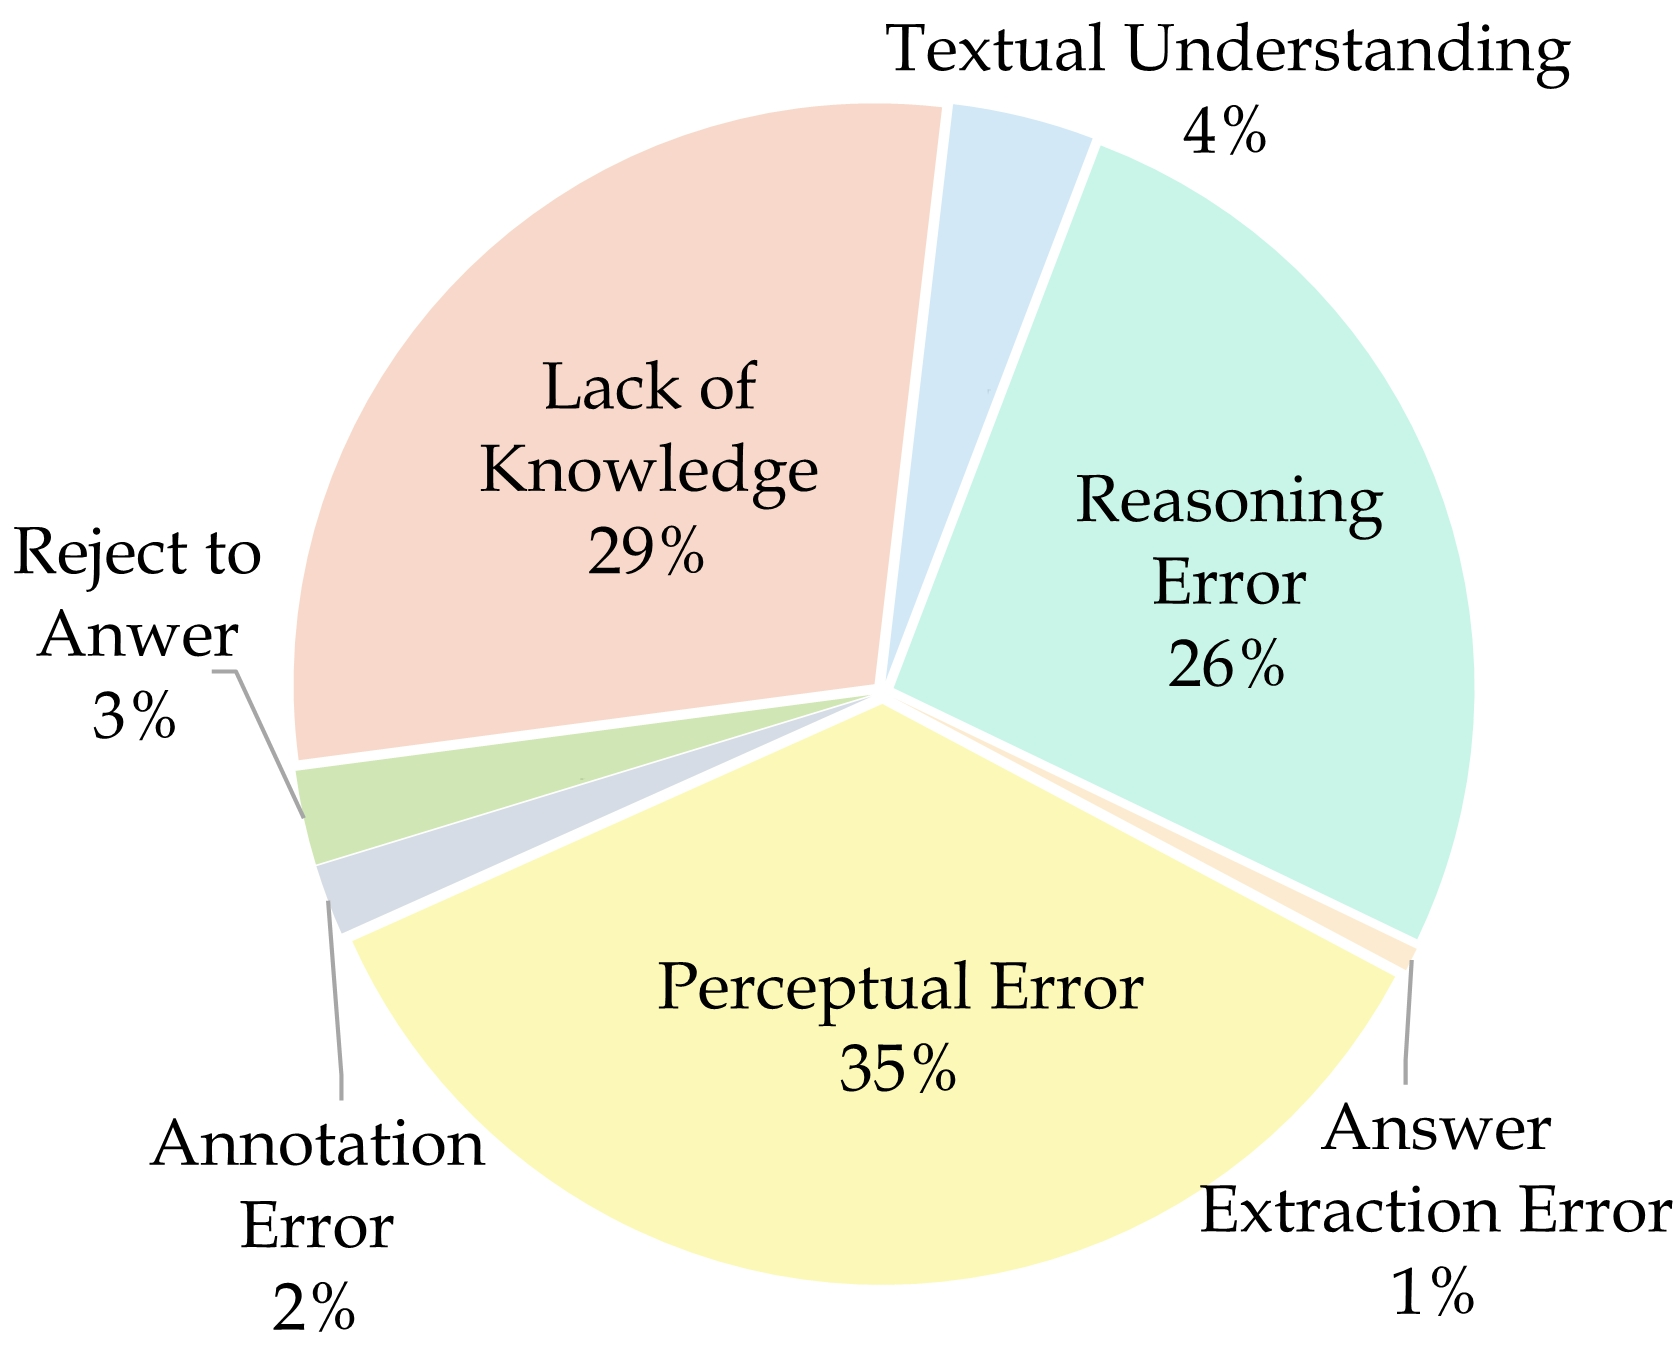
\includegraphics{mmmu_error_analysis.jpeg}}

\vspace{0.5em}
\small ``We meticulously examine 150 randomly sampled error instances from GPT-4V's predictions. These instances are analyzed by expert annotators who identify the root causes of mispredictions based on their knowledge and the golden explanations if available.''

\vfill
{\scriptsize Yue et al., ``MMMU: A Massive Multi-discipline Multimodal Understanding and Reasoning Benchmark for Expert AGI,'' CVPR 2024.}
\end{frame}

% Slide 9 - MMMU Pro vs ZeroBench bar chart
\begin{frame}{MMMU Pro vs ZeroBench (Sub)}
\centering
\begin{tikzpicture}
\begin{axis}[
    ybar=8pt,
    bar width=28pt,
    width=0.82\textwidth,
    height=0.68\textheight,
    ylabel={Score (\%)},
    ylabel style={font=\normalsize},
    title style={font=\large\bfseries, at={(0.5,1.05)}, anchor=south},
    symbolic x coords={GLM-4.5V (106B), Qwen3.6-35B-A3B},
    xtick=data,
    xticklabel style={font=\normalsize},
    yticklabel style={font=\small},
    ymin=0, ymax=90,
    ytick={0,10,20,30,40,50,60,70,80,90},
    ymajorgrids=true,
    grid style={dashed, gray!30},
    legend style={
        at={(0.5,-0.15)},
        anchor=north,
        legend columns=2,
        font=\normalsize,
        draw=none,
        fill=white,
        fill opacity=0.8,
        text opacity=1,
    },
    nodes near coords,
    nodes near coords align={vertical},
    every node near coord/.append style={font=\normalsize\bfseries, yshift=2pt},
    axis line style={gray!80},
    tick style={gray!80},
    enlarge x limits=0.5,
]
\addplot[fill=blue!50, draw=blue!70, rounded corners=1pt] coordinates {(GLM-4.5V (106B), 65.2) (Qwen3.6-35B-A3B, 75.3)};
\addplot[fill=orange!60, draw=orange!80, rounded corners=1pt] coordinates {(GLM-4.5V (106B), 23.4) (Qwen3.6-35B-A3B, 34.4)};
\legend{MMMU Pro, ZeroBench (sub)}
\end{axis}
\end{tikzpicture}

\vfill
{\scriptsize Data from GLM-4.5V Technical Report (2025) and Qwen Team, ``Qwen3.6-35B-A3B: Agentic Coding Power, Now Open to All,'' 2026.}
\end{frame}

\end{document}
